% =====================================================================
%  Round trips are not enough
%  URSS 2026 poster - A1 landscape - University of Warwick brand
%  Compile with pdflatex (Overleaf: set compiler to pdfLaTeX)
% =====================================================================
\documentclass[final]{beamer}
\usepackage[size=a1,orientation=landscape,scale=1.15]{beamerposter}
\usetheme{default}
\usecolortheme{default}
\beamertemplatenavigationsymbolsempty

\usepackage[T1]{fontenc}
\usepackage[utf8]{inputenc}
\usepackage{helvet}                 % Arial-metric sans, per Warwick brand
\renewcommand{\familydefault}{\sfdefault}
\usepackage{amsmath,amssymb,amsfonts}
\usepackage{tikz}
\usepackage{tcolorbox}
\usepackage{graphicx}
\usepackage{xcolor}
\usepackage{ragged2e}
\newcommand{\SPEEDUP}{7}
\newcommand{\WGAP}{65}
\newcommand{\TAUSPREAD}{6}
\newcommand{\OCCA}{0.35}
\newcommand{\OCCB}{0.042}
\newcommand{\LAMS}{10.0}
\newcommand{\LAMD}{10.0}
\newcommand{\DIMFALL}{1.3}

\setlength{\parindent}{0pt}
\setlength{\emergencystretch}{2em}
\usetikzlibrary{calc}
\tcbuselibrary{skins}

% ----------------------------------------------------------- palette
\definecolor{warwickblue}{HTML}{6CB7FF}   % brand panel blue
\definecolor{deepblue}{HTML}{1B5FB8}      % headings
\definecolor{ink}{HTML}{1A1C1F}
\definecolor{muted}{HTML}{535A61}
\definecolor{seoblue}{HTML}{3B5BDB}
\definecolor{deoorange}{HTML}{E8590C}
\definecolor{tint}{HTML}{EAF3FF}
\definecolor{warm}{HTML}{FFF4E6}
\definecolor{panelgrey}{HTML}{F2F4F6}
\definecolor{amber}{HTML}{9C5300}

\setbeamercolor{background canvas}{bg=white}
\setbeamercolor{normal text}{fg=ink}
\usebeamercolor[fg]{normal text}

% ------------------------------------------------- page furniture
% The blue strip, wordmark and crest sit at the same relative positions
% as the official Warwick A0 landscape template, scaled to A1.
\setbeamertemplate{background}{%
  \begin{tikzpicture}[remember picture,overlay]
    \fill[white] (current page.south west) rectangle (current page.north east);
    \fill[warwickblue]
      ($(current page.north west)+(0.9233\paperwidth,0)$)
      rectangle (current page.south east);
    \node[anchor=center,rotate=-90,inner sep=0pt] at
      ($(current page.north west)+(0.9638\paperwidth,-0.1122\paperheight)$)
      {
\includegraphics[width=0.1300\paperwidth]{figs/wordmark.png}};
    \node[anchor=south,inner sep=0pt] at
      ($(current page.south west)+(0.9638\paperwidth,0.0231\paperheight)$)
      {
\includegraphics[width=0.0611\paperwidth]{figs/crest.png}};
  \end{tikzpicture}%
}

% ------------------------------------------------------ typography
\setbeamerfont{block title}{size=\Large,series=\bfseries}
\setbeamercolor{block title}{fg=ink,bg=}
\setbeamercolor{block body}{fg=ink,bg=}
\setbeamertemplate{block begin}{%
  \vspace{0.4ex}%
  {\usebeamerfont{block title}\usebeamercolor[fg]{block title}\insertblocktitle}%
  \par\vspace{0.55ex}%
  \begin{beamercolorbox}[colsep*=0ex]{block body}%
  \justifying\setlength{\parskip}{0.7ex}%
}
\setbeamertemplate{block end}{\end{beamercolorbox}\vspace{1.2ex}}

\newcommand{\sechead}[2]{{\color{deepblue}\bfseries #1}\hspace{0.45em}#2}
\newcommand{\subhead}[1]{\vspace{0.3ex}{\large\bfseries #1}\par\vspace{0.5ex}}
\newcommand{\figcap}[1]{\vspace{-0.4ex}{\footnotesize\itshape\color{muted}#1}\par
  \vspace{1.1ex}}

\newtcolorbox{tintbox}[1][]{colback=tint,colframe=tint,boxrule=0pt,
  arc=1.5mm,left=5mm,right=5mm,top=3.5mm,bottom=3.5mm,#1}
\newtcolorbox{greybox}[1][]{colback=panelgrey,colframe=panelgrey,boxrule=0pt,
  arc=1.5mm,left=5mm,right=5mm,top=3.5mm,bottom=3.5mm,#1}
\newtcolorbox{warmbox}[1][]{colback=warm,colframe=warm,boxrule=0pt,
  arc=1.5mm,left=5mm,right=5mm,top=3.5mm,bottom=3.5mm,#1}

\newcommand{\algcomment}[1]{{\color{muted}\itshape #1}}

% margins: leave the blue strip clear on the right
\setbeamersize{text margin left=38mm,text margin right=112mm}

\newlength{\colw}
\setlength{\colw}{162mm}

\begin{document}
\begin{frame}[t]

% ================================================================ TITLE
\vspace{2mm}
{\fontsize{72}{80}\selectfont\bfseries Round trips are not enough\par}
\vspace{5mm}
{\fontsize{31}{36}\selectfont\color{deepblue}
 Efficiency of non-reversible parallel tempering on inhomogeneous
 multimodal targets\par}
\vspace{4mm}
{\fontsize{22}{26}\selectfont
 \textbf{Han Myo Htet}\;\;\textcolor{muted}{$\cdot$\;\;supervised by}\;
 Professor Krzysztof {\L}atuszy\'nski\;\;\textcolor{muted}{$\cdot$\;\;Department
 of Statistics, University of Warwick\;\;$\cdot$\;\;URSS 2026}\par}
\vspace{7mm}

\begin{columns}[t,totalwidth=\textwidth]

% ============================================================== COLUMN 1
\begin{column}{\colw}

\begin{block}{\sechead{1}{Sampling many modes}}
Posteriors in Bayesian inference and the loss surfaces of neural networks are
routinely \textbf{multimodal}. A single Metropolis chain settles into one mode
and then essentially never leaves it. Our benchmark makes the difficulty
explicit and controllable:
\vspace{-1.0ex}
\[
  \pi(x)\;=\;\tfrac12\,\mathcal N\!\left(\mathbf 1_d,\,s_1^2 I\right)
        \;+\;\tfrac12\,\mathcal N\!\left(-\mathbf 1_d,\,s_2^2 I\right),
  \qquad x\in\mathbb R^{d}.
\]
\vspace{-2.6ex}

Both modes carry weight exactly $\tfrac12$. When $s_1=s_2$ the target is
\emph{homogeneous}; when $s_1\neq s_2$ the two modes have different shapes, and
that single difference is what the whole poster is about.

\textbf{Parallel tempering} runs $N$ chains along a temperature ladder
$1=\beta_0>\beta_1>\dots>\beta_{N-1}=\beta_{\min}$, chain $j$ targeting
\vspace{-1.0ex}
\[
  \pi_{\beta_j}(x)\;\propto\;\pi(x)^{\beta_j}.
\]
\vspace{-2.6ex}

Flattened chains cross barriers easily; swap moves pass that mobility down to
the cold chain $\beta_0=1$, which is the one we keep.
\end{block}

\begin{block}{\sechead{2}{The two schedules}}
\vspace{-0.8ex}
\begin{tcolorbox}[colback=white,colframe=muted!30,boxrule=0.7pt,
  arc=1.5mm,left=4mm,right=4mm,top=3mm,bottom=3mm]
{\bfseries Algorithm 1}\hspace{0.8em}One parallel tempering scan
\par\vspace{1.6ex}
\begin{tabular}{@{}r@{\hspace{0.8em}}l@{}}
{\color{muted}\small 1} & \textbf{input:} ladder $\beta$, states
   $x_0,\dots,x_{N-1}$, scan index $i$ \\[0.4ex]
{\color{muted}\small 2} & \textbf{for} $j=0,\dots,N-1$ \textbf{in parallel}
   \\[0.4ex]
{\color{muted}\small 3} & \quad\textbf{for} $t=1,\dots,T$ \\[0.4ex]
{\color{muted}\small 4} & \quad\quad $y\sim\mathcal N\!\big(x_j,\,
   (r^2/\beta_j)I\big)$ \\[0.4ex]
{\color{muted}\small 5} & \quad\quad $x_j\leftarrow y$ \ w.p. \
   $1\wedge\big(\pi(y)/\pi(x_j)\big)^{\beta_j}$ \\[1.1ex]
{\color{muted}\small 6} & \textcolor{seoblue}{\textbf{SEO}}\, :\;
   $p\sim\mathrm{Bernoulli}(1/2)$ \\[0.4ex]
{\color{muted}\small 7} & \textcolor{deoorange}{\textbf{DEO}}\, :\;
   $p\leftarrow i \bmod 2$ \\[1.1ex]
{\color{muted}\small 8} & \textbf{for} $j=p,\,p+2,\dots\le N-2$ \\[0.4ex]
{\color{muted}\small 9} & \quad swap $x_j\leftrightarrow x_{j+1}$ \ w.p. \
   $1\wedge A_j$ \\[0.4ex]
{\color{muted}\small 10} & record the chain each replica now occupies \\
\end{tabular}
\end{tcolorbox}
\vspace{0.6ex}

The two schemes differ only in \textbf{lines 6--7}. The swap
acceptance ratio is
\vspace{-1.0ex}
\begin{align*}
  A_j&=\frac{\pi(x_j)^{\beta_{j+1}}\pi(x_{j+1})^{\beta_j}}
           {\pi(x_j)^{\beta_j}\pi(x_{j+1})^{\beta_{j+1}}}\\[0.6ex]
     &=\exp\!\big\{(\beta_{j+1}-\beta_j)
       \big[\log\pi(x_j)-\log\pi(x_{j+1})\big]\big\}.
\end{align*}
\vspace{-2.6ex}

Under \textcolor{seoblue}{\textbf{SEO}} the parity is random, so a replica's
position on the ladder performs a \emph{random walk} and needs order $N^2$
scans to cross it. Under \textcolor{deoorange}{\textbf{DEO}} the parity
alternates deterministically, replicas move \emph{ballistically}, and they
cross in order $N$ scans~[1].
\end{block}

\vspace{-1.0ex}
\begin{warmbox}
{\small\textbf{\textcolor{amber}{A NOTE ON IMPLEMENTATION}}}\par\vspace{1.2ex}
{\small Forming $A_j$ or the local acceptance ratio from densities rather than
\emph{log} densities underflows at $d=30$: below $\beta\approx0.02$ both
$\pi(x)$ and $\pi(y)$ evaluate to exactly zero, the ratio becomes $0/0$, and
the hottest ${\sim}15\%$ of the ladder silently accepts every proposal. All
results here use log densities.}
\end{warmbox}


\end{column}

% ============================================================== COLUMN 2
\begin{column}{\colw}

\begin{block}{\sechead{3}{What the theory promises}}
Write $s_j$ for the acceptance rate of the swap between chains $j$ and $j+1$,
and $r_j=1-s_j$ for the rejection rate. Syed et al.~[1] show efficiency is
governed by the \textbf{communication barrier}
\vspace{-1.0ex}
\[
  \Lambda=\sum_{j=0}^{N-2} r_j
  \;\xrightarrow[\ N\to\infty\ ]{}\;
  \int_{\beta_{\min}}^{1}\lambda(\beta)\,\mathrm d\beta ,
\]
\vspace{-2.6ex}

a property of the temperature \emph{path}, not of the schedule. With the
schedule inefficiency $E=\sum_j r_j/s_j$, the \textbf{round trip rate} $\tau$
— complete target $\to$ reference $\to$ target excursions per scan — obeys
\vspace{-1.0ex}
\begin{align*}
  \tau_{\mathrm{SEO}}&=\frac{1}{2N+2E},
  \qquad
  \tau_{\mathrm{DEO}}=\frac{1}{2+2E},\\[1.0ex]
  \tau_{\mathrm{DEO}}&\;\xrightarrow[\ N\to\infty\ ]{}\;
  \bar\tau=\frac{1}{2+2\Lambda}.
\end{align*}
\vspace{-2.6ex}

So refining the ladder drives $\tau_{\mathrm{SEO}}$ to zero like $1/N$, while
$\tau_{\mathrm{DEO}}$ approaches a limit \textbf{independent of $N$}, maximised
at $N\approx 2\Lambda$. That is the promise of non-reversibility, and the
thing we set out to test.
\end{block}

\vspace{-0.6ex}
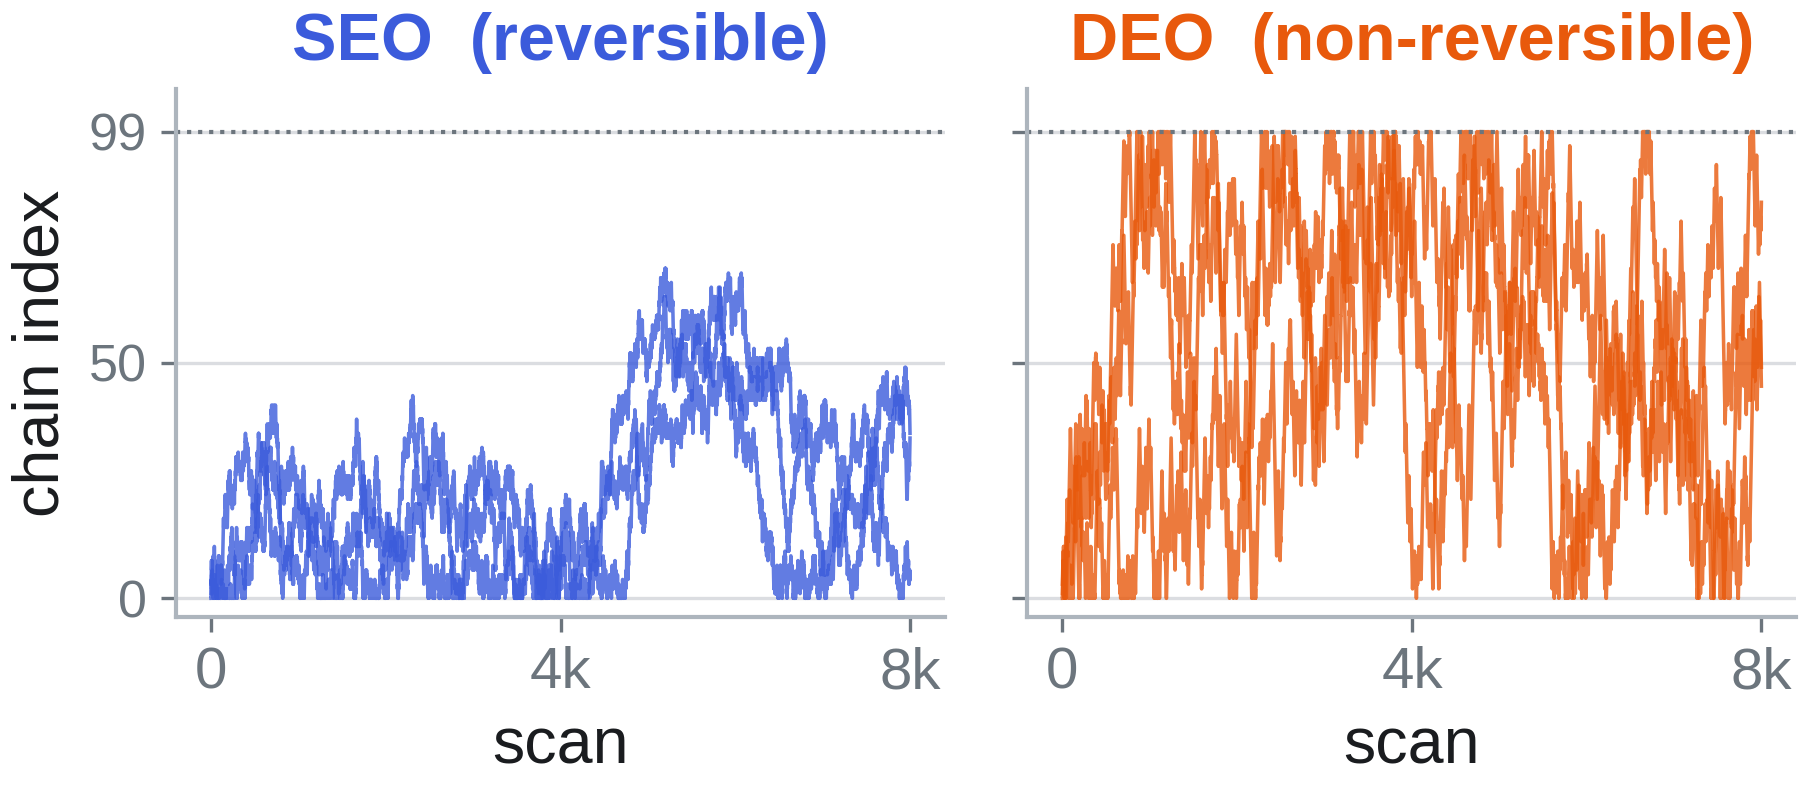
\includegraphics[width=\colw]{figs/fig_1_index.png}
\figcap{Chain index 0 is the target, 99 the reference. Under DEO a replica sweeps
the whole ladder; under SEO it diffuses near the cold end and rarely reaches
the top.}

\begin{greybox}
{\small\textbf{\textcolor{muted}{THE EXPERIMENT}}}\par\vspace{1.2ex}
{\small $d=30$ \;$\cdot$\; $s_1=0.3$ (mode A, at $+\mathbf 1$) \;$\cdot$\;
$s_2=0.4$ (mode B, at $-\mathbf 1$) \;$\cdot$\; $N=100$ chains \;$\cdot$\;
$\beta$ geometric on $[0.01,1]$ \;$\cdot$\; $r=0.15$, $T=8$ \;$\cdot$\;
every chain started in mode B \;$\cdot$\; densities evaluated in
\textbf{log space}.}
\end{greybox}
\vspace{2.2ex}

\begin{block}{\sechead{4}{The speed-up is real}}
\vspace{-0.4ex}
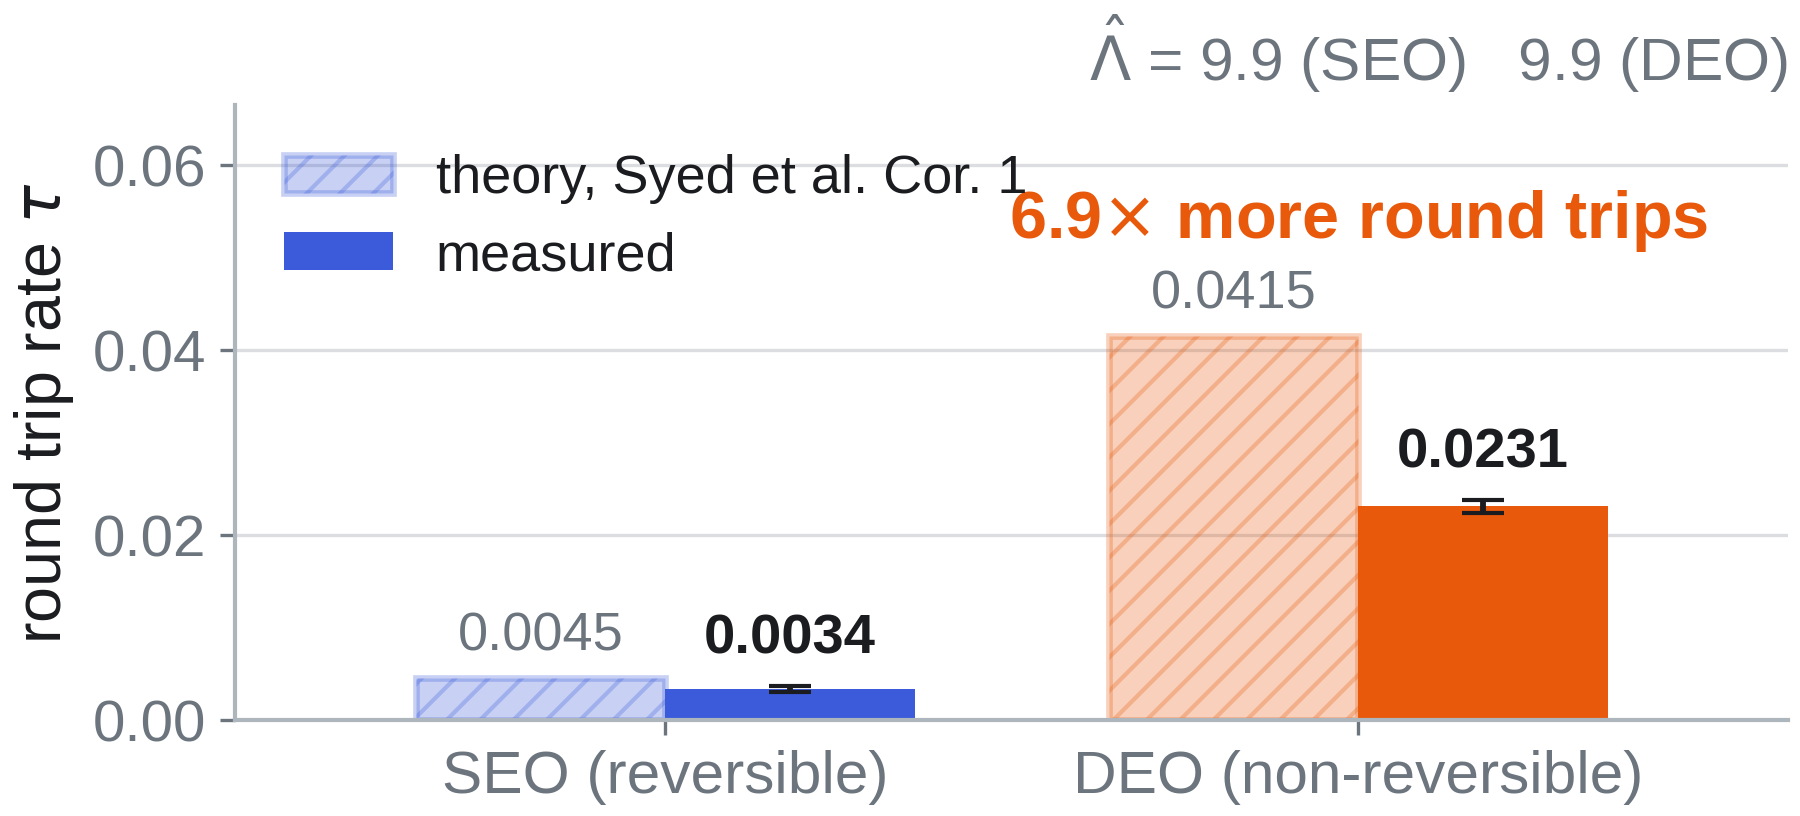
\includegraphics[width=\colw]{figs/fig_2_speedup.png}
\vspace{0.6ex}

Both schedules recover the \textbf{same barrier}, as they must. DEO completes
\textbf{\SPEEDUP$\times$ more round trips}. Both rates sit below the
Corollary~1 values, which an optimally tuned ladder attains at stationarity;
the qualitative prediction holds clearly.
\end{block}

\end{column}

% ============================================================== COLUMN 3
\begin{column}{\colw}

\begin{block}{\sechead{5}{But the samples are wrong}}
\vspace{-0.4ex}
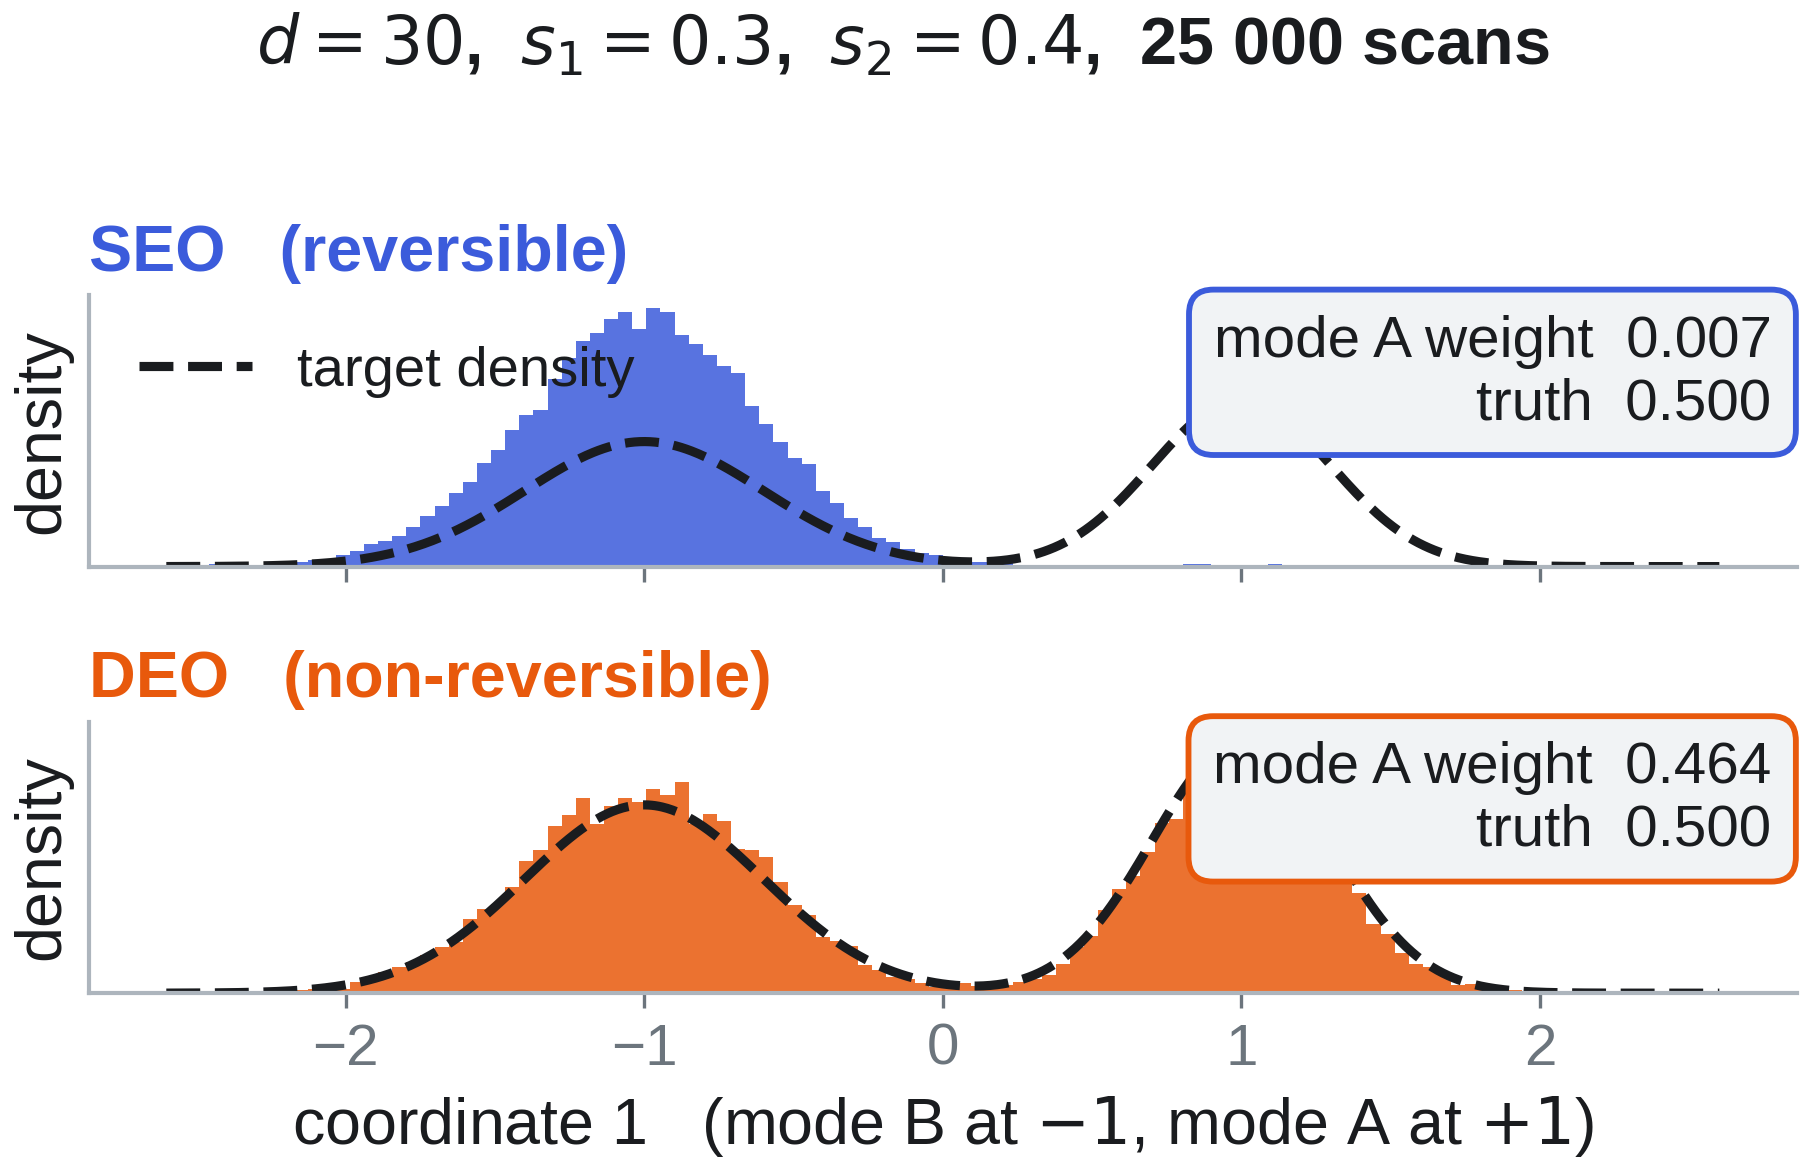
\includegraphics[width=\colw]{figs/fig_3_failure.png}
\vspace{0.6ex}

Same target, same budget, same ladder. SEO never escapes the mode it started
in; DEO does. Yet the round trip rate separates the two by a factor of
\SPEEDUP, while the recovered mode weight separates them by a factor of
\WGAP. \textbf{$\tau$ does not predict the gap it is meant to explain.}
\end{block}

\begin{block}{\sechead{6}{A controlled test}}
Hold the algorithm, the ladder and the budget fixed, and turn one knob: the
\textbf{inhomogeneity} $s_2/s_1$, from $1$ (identical modes) to $4/3$. Both
modes keep weight $\tfrac12$ throughout — the right answer never moves.
\vspace{0.8ex}

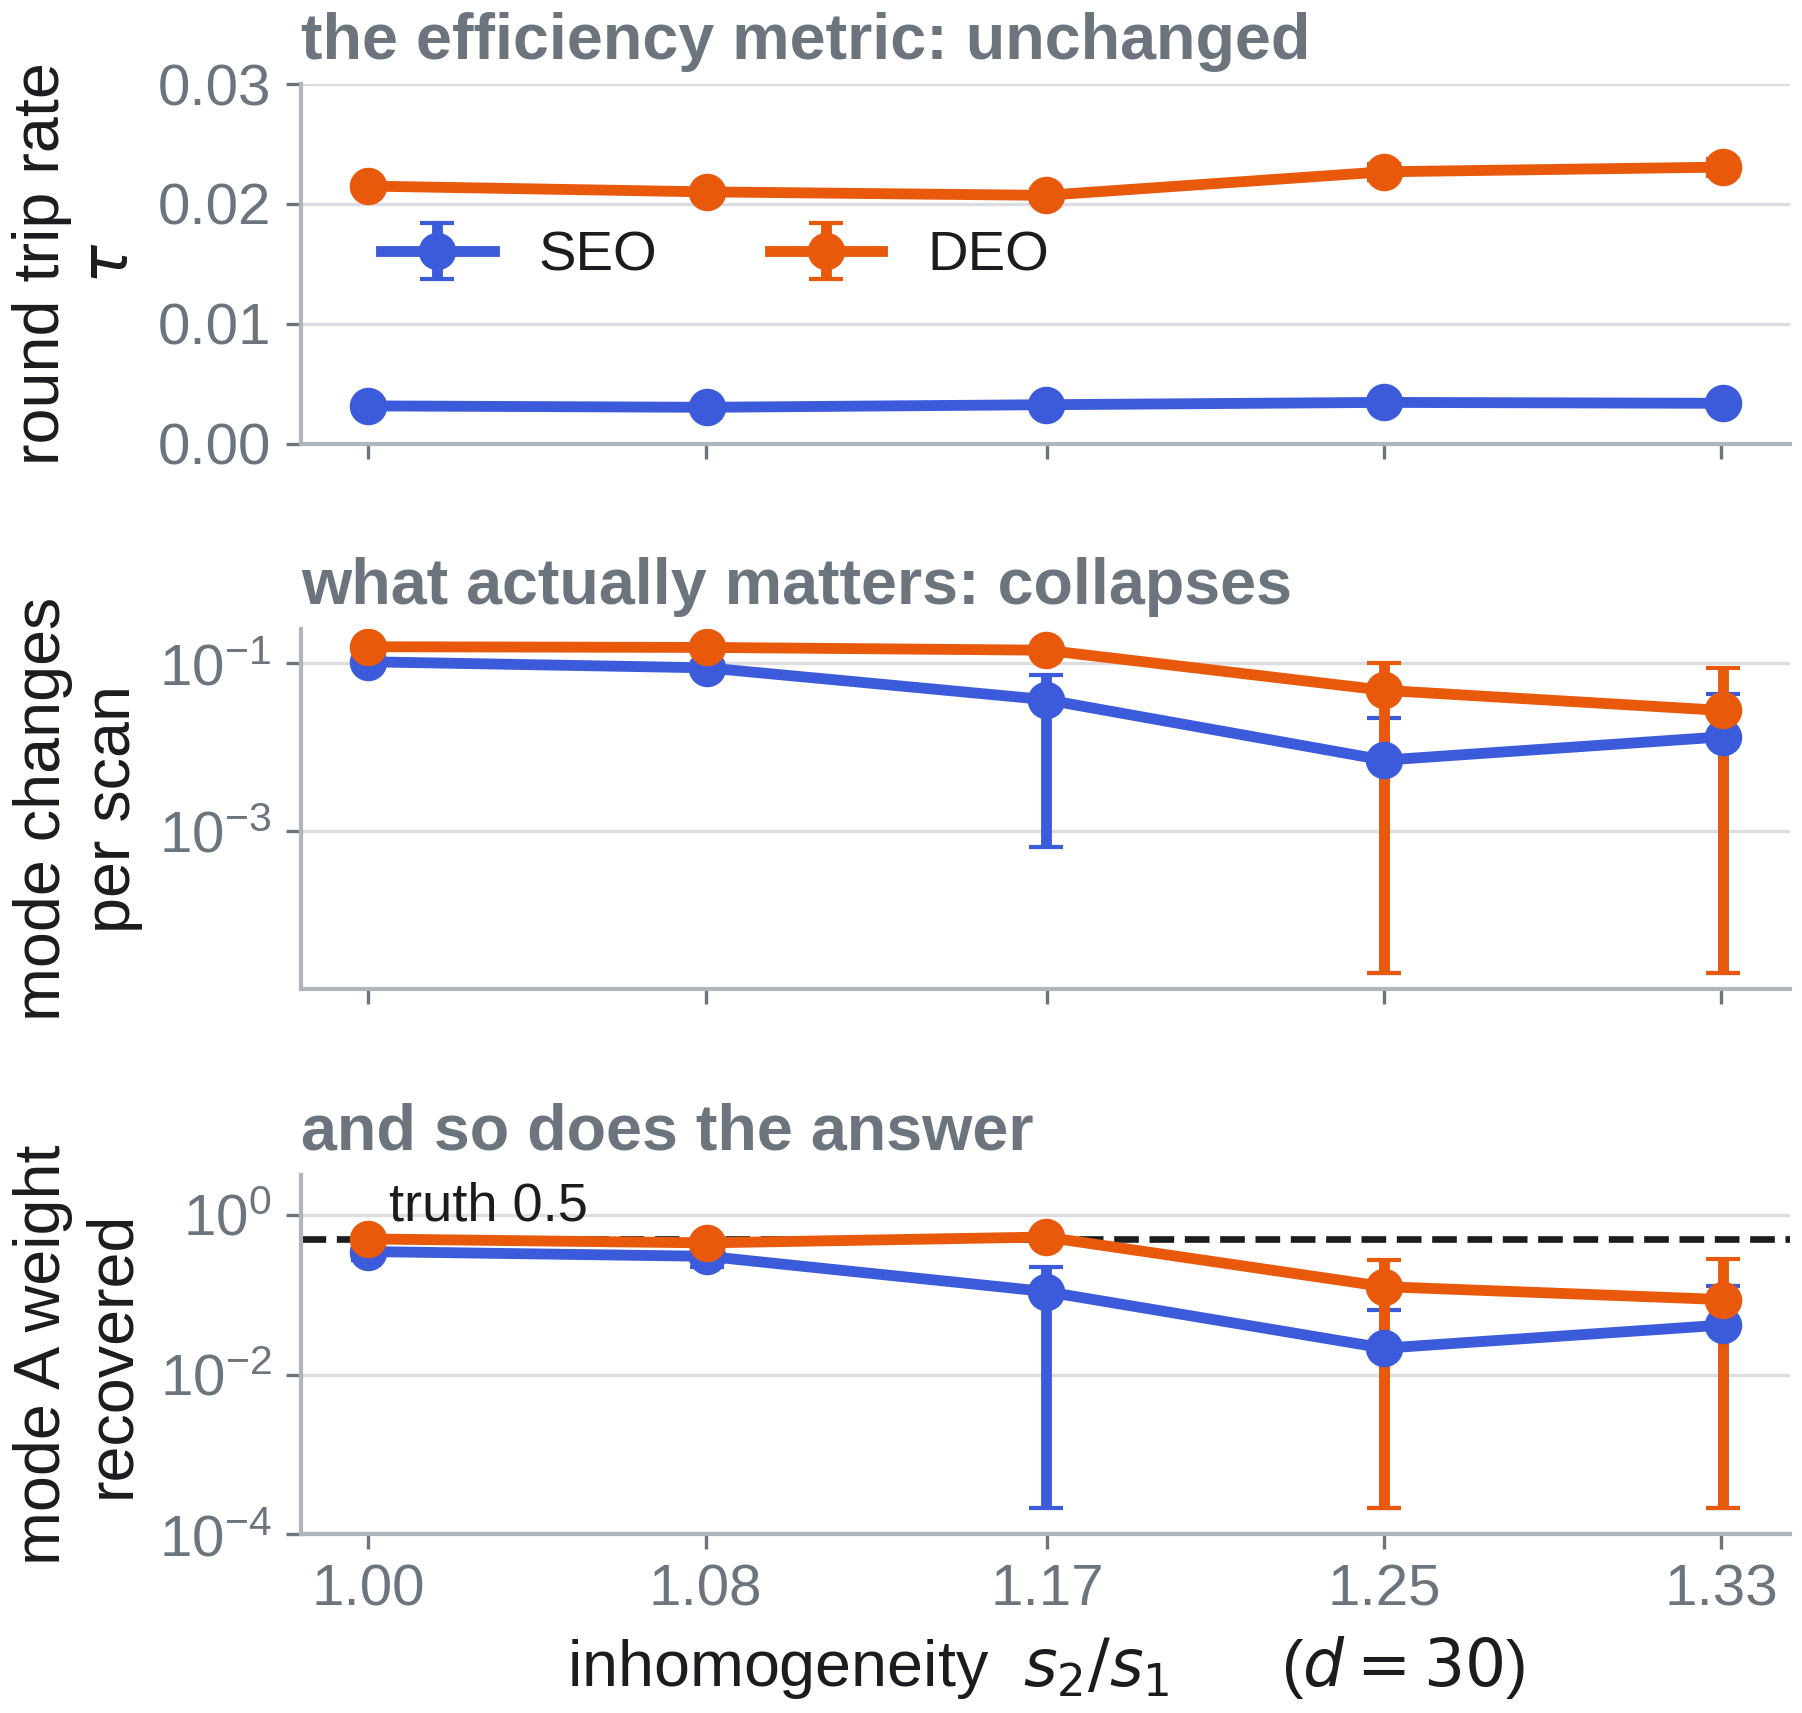
\includegraphics[width=\colw]{figs/fig_5_sweep.png}
\figcap{Mean over 6 independent runs of 20\,000 scans; bars are $\pm1$ s.d.}

The round trip rate is \textbf{flat to within $\pm$\TAUSPREAD\%} across the
sweep, for both schedules, while the recovered weight of mode A falls from
\OCCA{} to \OCCB{} under SEO. Judged by its own diagnostic the sampler is in
identical health at both ends. \textbf{The metric cannot see the difficulty
it is meant to measure.}
\end{block}

\end{column}

% ============================================================== COLUMN 4
\begin{column}{\colw}

\begin{block}{\sechead{7}{Why the metric is blind}}
Take the modes well separated and apply Laplace's approximation to
$\pi^\beta$. Near mode $i$,
\vspace{-1.0ex}
\[
  \pi(x)^{\beta}\;\approx\;
  \Big[\tfrac12(2\pi s_i^2)^{-d/2}\Big]^{\beta}
  \exp\!\Big\{-\tfrac{\beta}{2s_i^2}\|x-\nu_i\|^2\Big\},
\]
\vspace{-2.6ex}

a Gaussian of variance $s_i^2/\beta$. Integrating gives mass proportional to
$(s_i^2)^{-d\beta/2}(s_i^2/\beta)^{d/2}$; the $\beta$ factors cancel in the
ratio and
\vspace{-0.6ex}
\begin{tintbox}
\centering
$\displaystyle
  \frac{\pi_\beta(\mathrm A)}{\pi_\beta(\mathrm B)}
  =\left(\frac{s_1}{s_2}\right)^{\,d\,(1-\beta)}$
\end{tintbox}
\vspace{1.4ex}

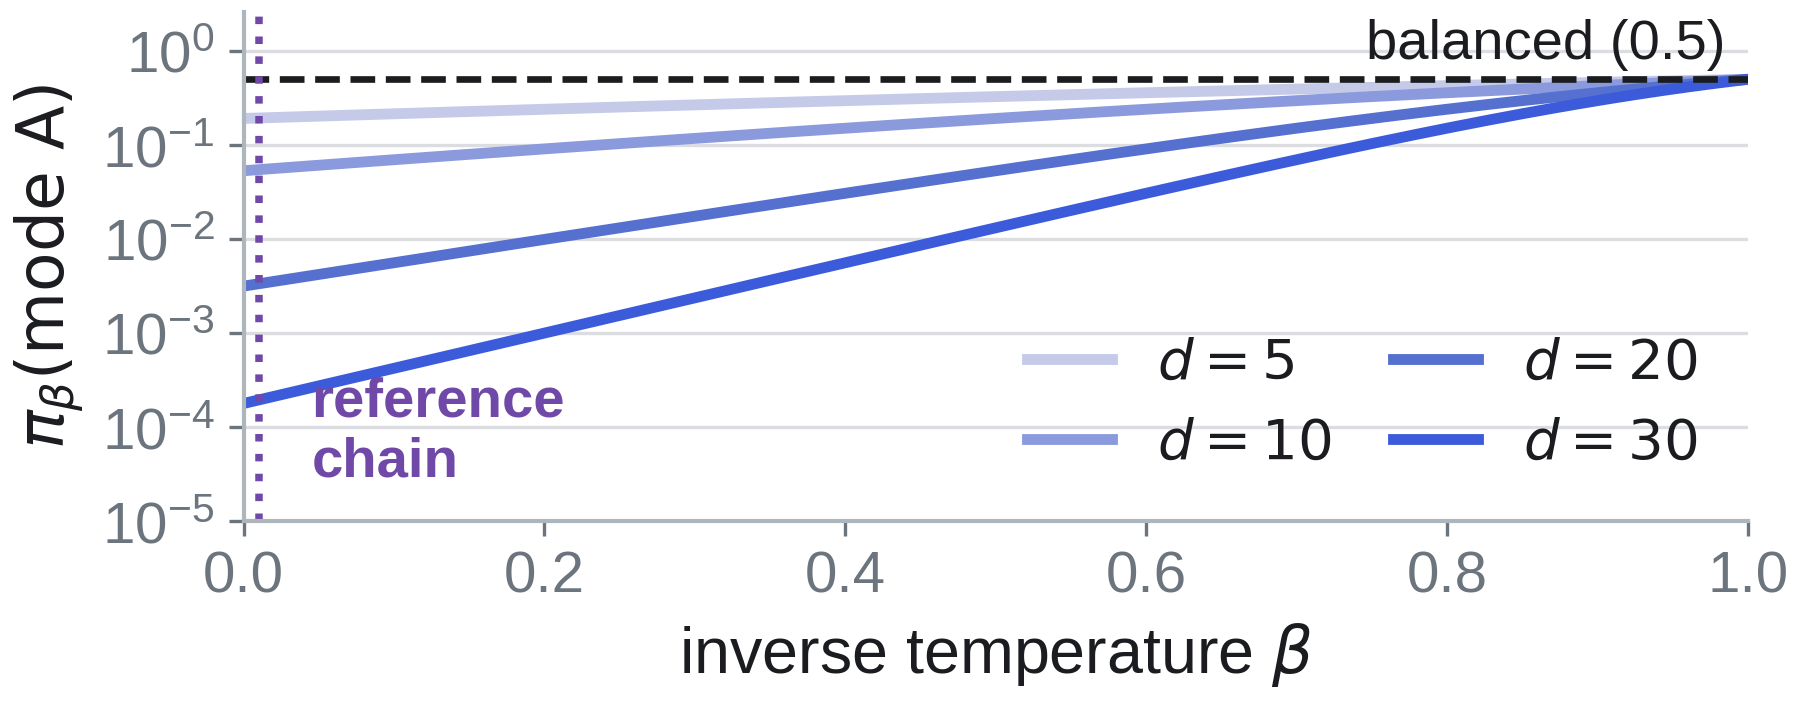
\includegraphics[width=\colw]{figs/fig_4_closedform.png}
\vspace{0.6ex}

Only at $\beta=1$ are the modes balanced, and the imbalance is
\textbf{exponential in $d(1-\beta)$}: at $d=30$ the reference chain gives mode
A a weight of $1.9\times10^{-4}$ instead of $\tfrac12$. A replica that climbs
the whole ladder is therefore very likely to come back down into the mode it
left: round trips are plentiful, \textbf{useful} round trips are not. This is
the mechanism behind the torpid-mixing bounds of Woodard et al.~[2].
\end{block}

\begin{block}{\sechead{8}{Blindness in dimension}}
\vspace{-0.4ex}
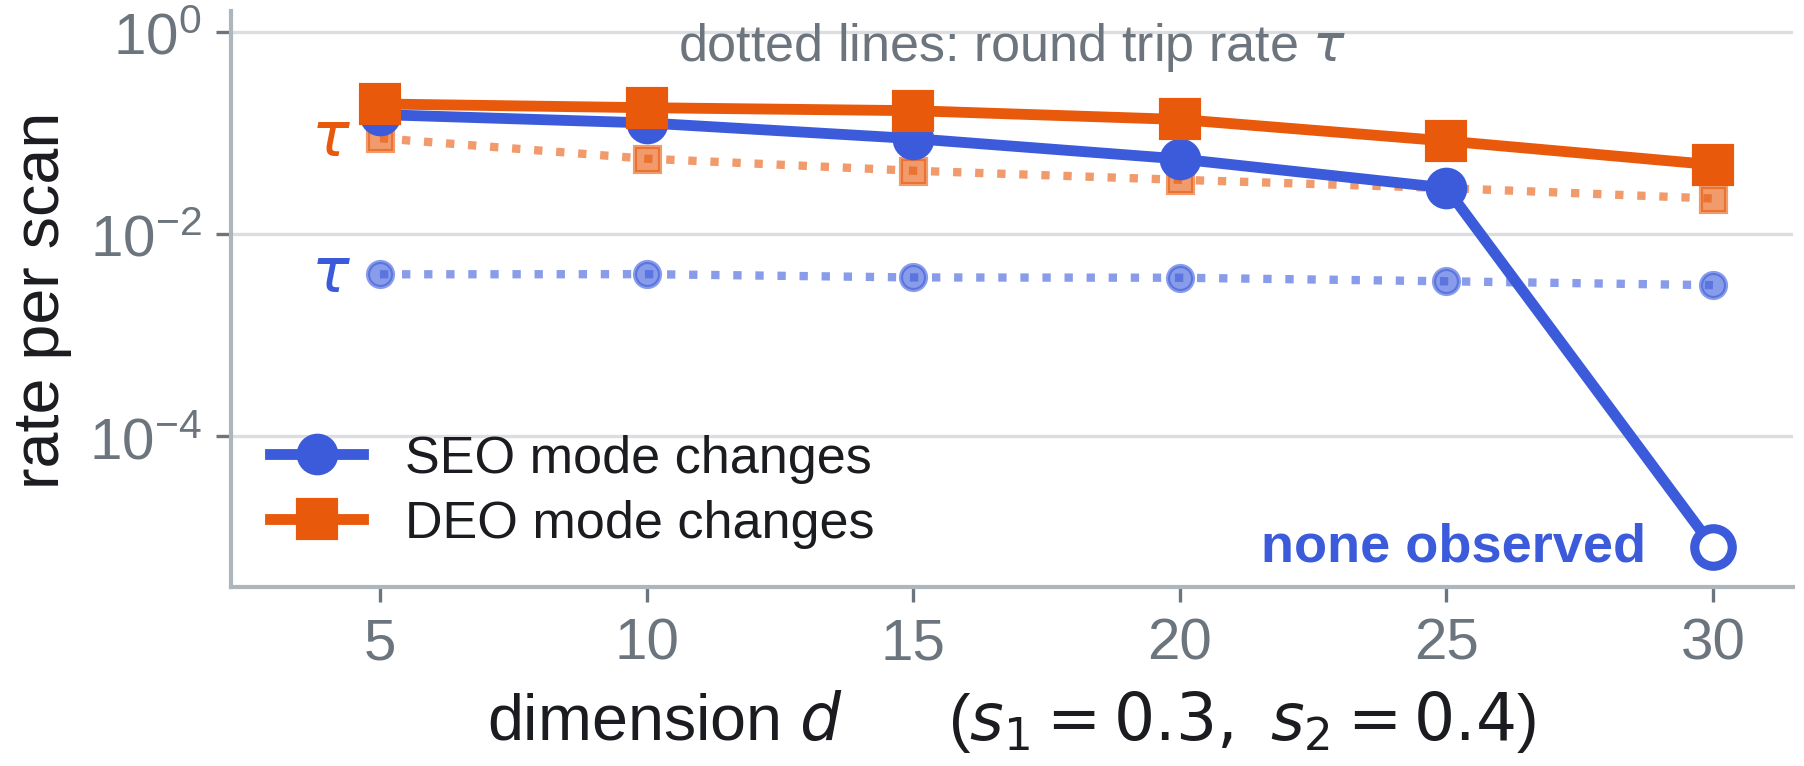
\includegraphics[width=\colw]{figs/fig_6_dimension.png}
\vspace{0.4ex}

Fix $s_2/s_1=4/3$ and raise $d$ instead. The SEO round trip rate falls by only
$\DIMFALL\times$, while its mode-change rate falls to zero: in four runs of
20\,000 scans at $d=30$ the cold chain never once changed basin.
\end{block}

\begin{block}{\sechead{9}{Conclusions}}
\textbf{The non-reversible speed-up is real} — an order-of-magnitude gain in
round trips, as advertised.

\textbf{$\tau$ and $\Lambda$ describe the ladder, not the target}, staying flat
where the sampler goes from working to failing outright.

\textbf{Refining the ladder cannot repair this} — the imbalance belongs to the
path, not its discretisation.

\textbf{Report a mode-aware diagnostic alongside $\tau$} — how often the cold
chain actually changes basin.
\end{block}



\end{column}
\end{columns}

% ========================================================== REFERENCES
\vspace{2mm}
{\footnotesize\color{muted}
\textbf{[1]} Syed, Bouchard-C\^ot\'e, Deligiannidis \& Doucet (2022).
Non-reversible parallel tempering: a scalable highly parallel MCMC scheme.
\emph{JRSS-B} 84(2), 321--350.\quad
\textbf{[2]} Woodard, Schmidler \& Huber (2009). Sufficient conditions for
torpid mixing of parallel and simulated tempering. \emph{SPA} 119(6).\quad
\textbf{[3]} Roberts \& Rosenthal (2023). Quantifying the speed-up from
non-reversibility in MCMC tempering algorithms.\quad
\textbf{[4]} Chatterjee (2023). Spectral gap of non-reversible Markov chains.
\par}

\end{frame}
\end{document}
